%-----------------------------------------------------------------------------------------------------------------------------------------------------------------------------------------------
% Resultados/Discussões: 
% Aqui se mostra o que o trabalho permitiu produzir, e às vezes o que pode ser comparado com outros trabalhos
% Aqui ficam claras se as propostas do trabalho são relevantes ou não, pois devem permitir a discussão do trabalho;
% Deve-se responder: Os resultados estão claros em bom número (nem muito nem pouco) que permitam avaliar realmente a proposta e o que foi produzido.
\chapter{Resultados}
\label{Resultados}

Os resultados apresentados neste capítulo estão inteiramente relacionados as funções fundamentais presentes na interface gráfica desenvolvida. Além disso, tem-se presente a seção que apresenta 
os dados obtidos através dos testes de desempenho dos métodos de \textit{Stereo Matching} nas plataformas utilizadas.


%-----------------------------------------------------------------------------------------------------------------------------------------------------------------------------------------------
\section{Interface Gráfica - \textit{StereoVisionGUI}}

Nesta seção, o software desenvolvido apresenta uma interface gráfica (GUI -- \textit{Graphical User Interface}) amigável, a qual facilita a visualização das imagens da câmera estéreo, 
dos mapas de disparidades, da reconstrução tridimensional e do método de processamento de imagens desenvolvido. Atualmente, o software conta com três métodos para encontrar correspondências 
estéreo (BM, SGBM e BMGPU) e com 8 opções das quais 6 delas são destinadas a visualização das seguintes perspectivas:

\begin{enumerate}
  \item Imagens retificadas das câmeras esquerda e direita
  \item Mapa de disparidade em Escala de Cinza e RGB
  \item Mapa tridimensional do ambiente reconstruído em Escala de Cinza e RGB
  \item Imagem da Câmera Esquerda com o indicador de objeto rastreado e Imagem binária resultante da limiarização por distância.
  \item Imagem resultante do processo de detecção de movimentos e Imagem resultante do processo de detecção de movimentos limiarizada por distância. 
  \item Imagem resultante da adição da imagem à direita com a Imagem da Câmera Esquerda e Imagem resultante do processo de realce das bordas dos objetos em movimento próximos ao veículo.
\end{enumerate} 

O botão \textit{Show Left/Right} seleciona a opção na qual a interface gráfica permite a visualização simultânea das imagens retificadas de ambas câmera. A figura \ref{gui_showleftright_view} 
ilustra o comportamento do software quando essa opção é selecionada. 

\begin{figure}[H]
 	\centering
 	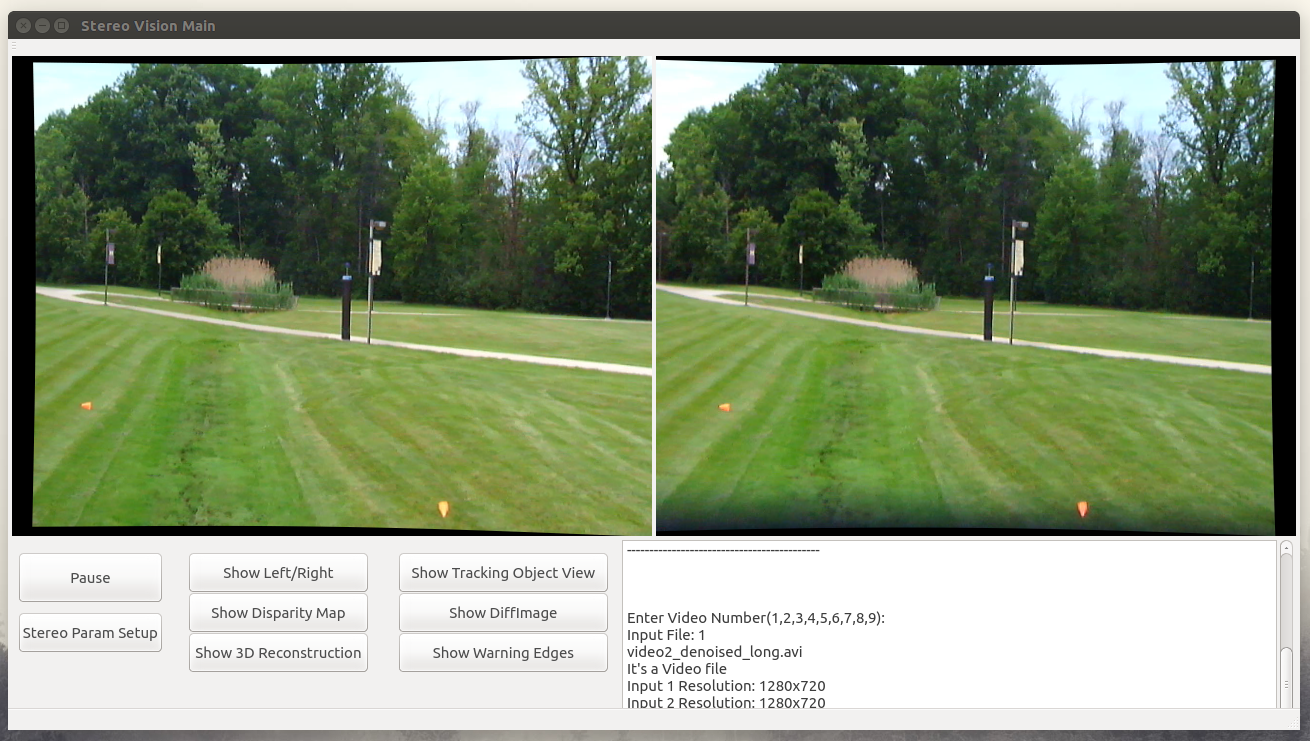
\includegraphics[scale=0.35]{./Resources/gui_showleftright_view.png}
 	\caption{Interface Gráfica - Visualização simultânea dos quadros das câmeras esquerda e direita}
 	\label{gui_showleftright_view}
\end{figure}

O botão \textit{Show Disparity Map} seleciona a opção na qual a interface gráfica permite a visualização simultânea dos mapas de disparidade em escala de cinza e RGB. A figura 
\ref{gui_showdisparitymap_view} ilustra o comportamento do software quando essa opção é selecionada. 

\begin{figure}[H]
 	\centering
 	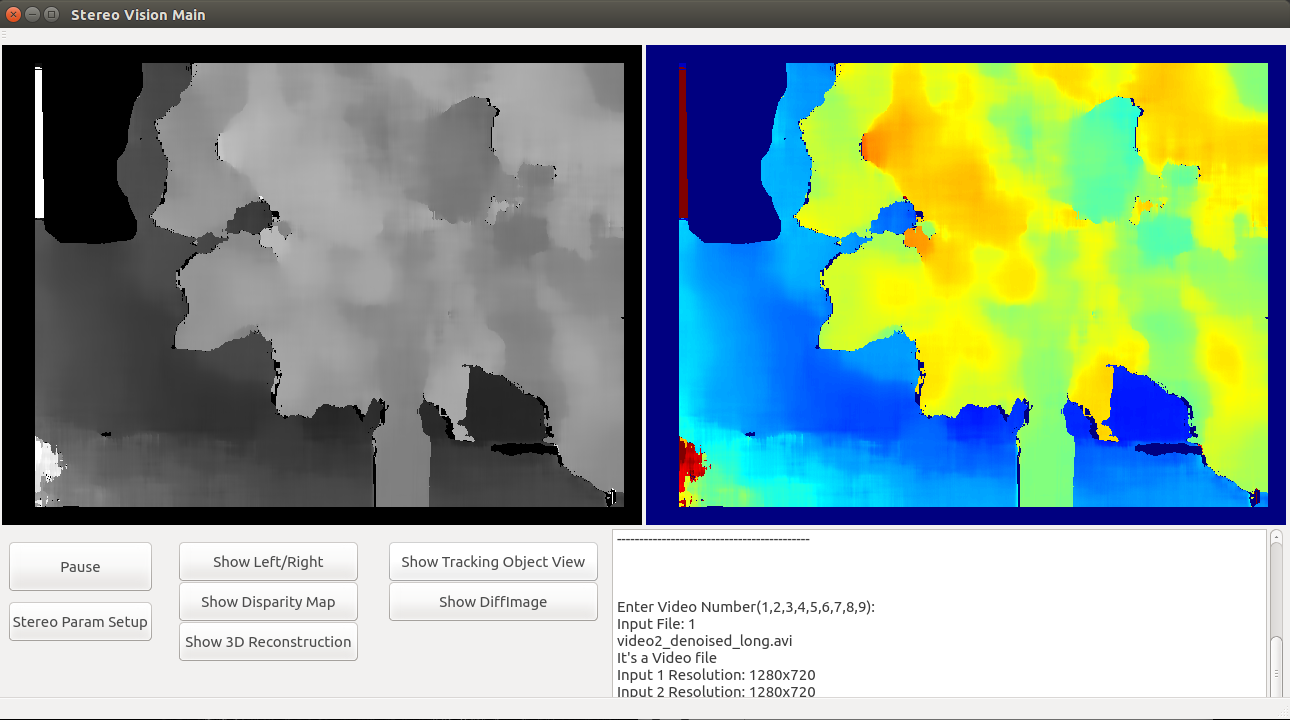
\includegraphics[scale=0.35]{./Resources/gui_showdisparitymap_view.png}
 	\caption{Interface Gráfica - Visualização dos Mapa de disparidade em Escala de Cinza e RGB}
 	\label{gui_showdisparitymap_view}
\end{figure}

O botão \textit{Show 3D Reconstruction} seleciona a opção na qual a interface gráfica permite a visualização simultânea dos mapas tridimensionais do ambiente reconstruído em escala de cinza e 
RGB. A figura \ref{gui_show3dreconstruction_view} ilustra o comportamento do software quando essa opção é selecionada. 

\begin{figure}[H]
 	\centering
 	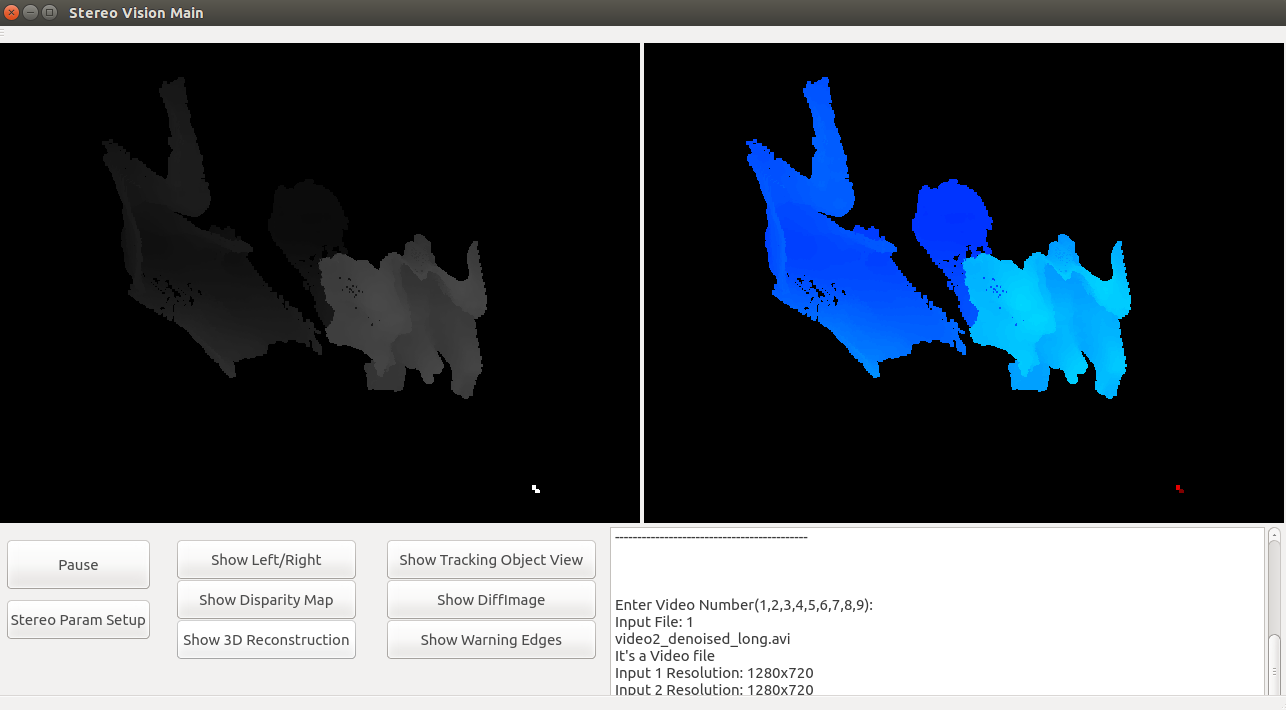
\includegraphics[scale=0.35]{./Resources/gui_show3dreconstruction_view.png}
 	\caption{Interface Gráfica - Visualização dos Mapa de disparidade em Escala de Cinza e RGB}
 	\label{gui_show3dreconstruction_view}
\end{figure}

O botão \textit{Show Tracking Object View} seleciona a opção na qual a interface gráfica permite a visualização simultânea da imagem da câmera Esquerda com o indicador de objeto rastreado e 
imagem binária resultante da limiarização por distância. A figura \ref{gui_show_tracking_object_view} ilustra o comportamento do software quando essa opção é selecionada. 

\begin{figure}[H]
 	\centering
 	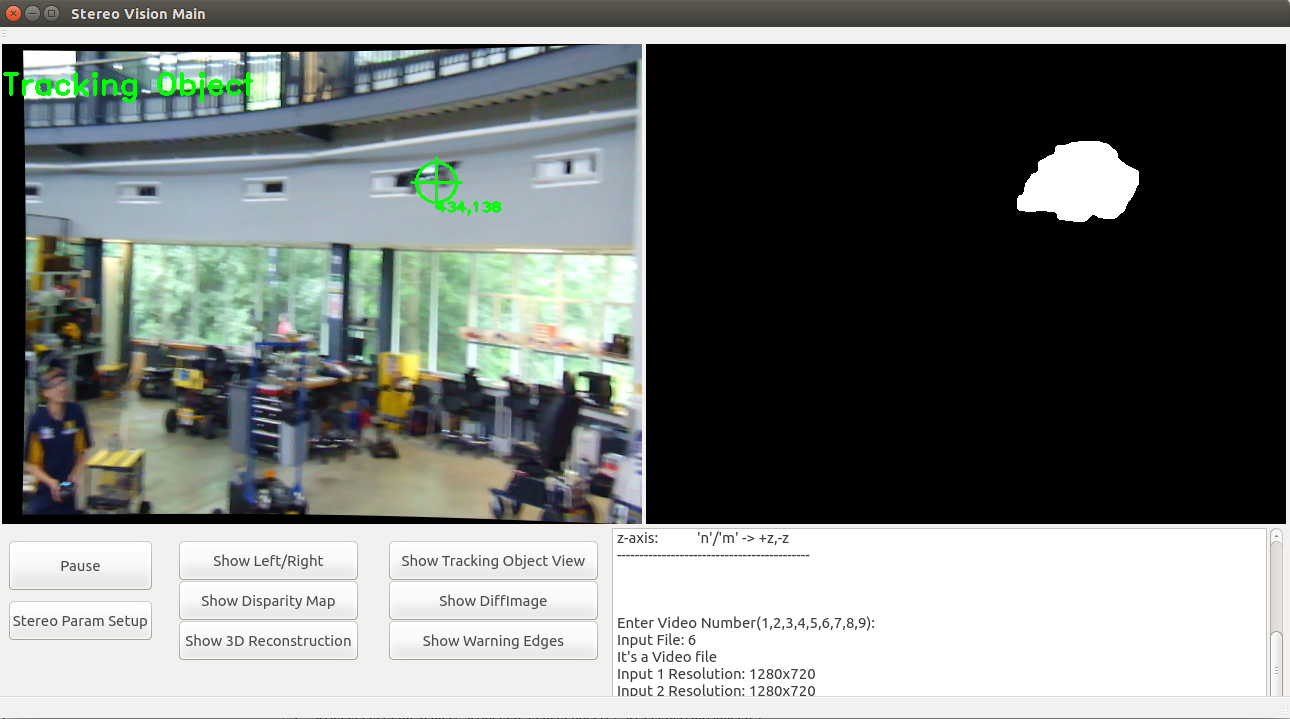
\includegraphics[scale=0.35]{./Resources/gui_show_tracking_object_view.png}
 	\caption{Interface Gráfica - Visualização da Imagem da Câmera Esquerda com o indicador de objeto rastreado e da Imagem binária resultante da limiarização por distância}
 	\label{gui_show_tracking_object_view}
\end{figure}

O botão \textit{Show DiffImage} seleciona a opção na qual a interface gráfica permite a visualização simultânea da imagem resultante do processo de detecção de movimentos e imagem resultante do 
processo de detecção de movimentos limiarizada por distância. A figura \ref{gui_showdiffimage_view} ilustra o comportamento do software quando essa opção é selecionada. 

\begin{figure}[H]
 	\centering
 	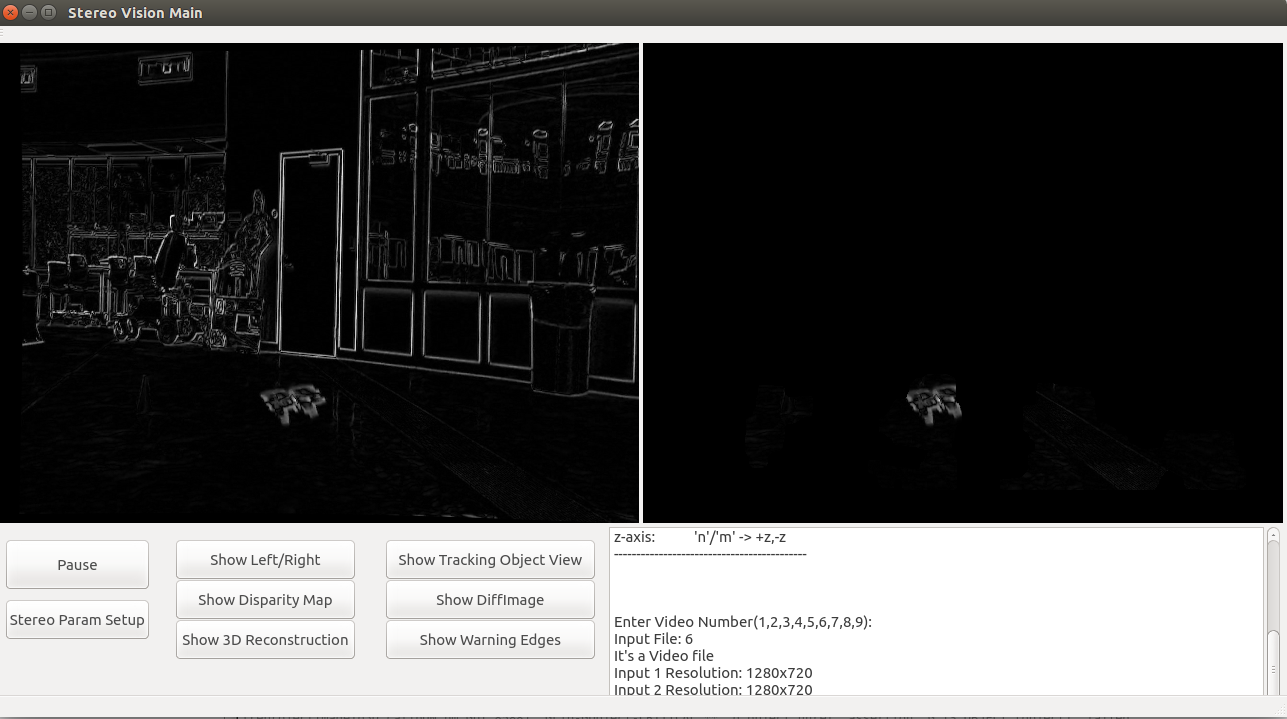
\includegraphics[scale=0.35]{./Resources/gui_showdiffimage_view.png}
 	\caption{Interface Gráfica - Visualização da imagem resultante do processo de detecção de movimentos e imagem resultante do processo de detecção de movimentos limiarizada por distância}
 	\label{gui_showdiffimage_view}
\end{figure}

O botão \textit{Show DiffImage} seleciona a opção na qual a interface gráfica permite a visualização simultânea da imagem resultante da adição da imagem à direita com a imagem da câmera esquerda 
e imagem resultante do processo de realce das bordas dos objetos em movimento próximos ao veículo. A figura \ref{gui_showwarningedges_view} ilustra o comportamento do software quando essa opção 
é selecionada. 

\begin{figure}[H]
 	\centering
 	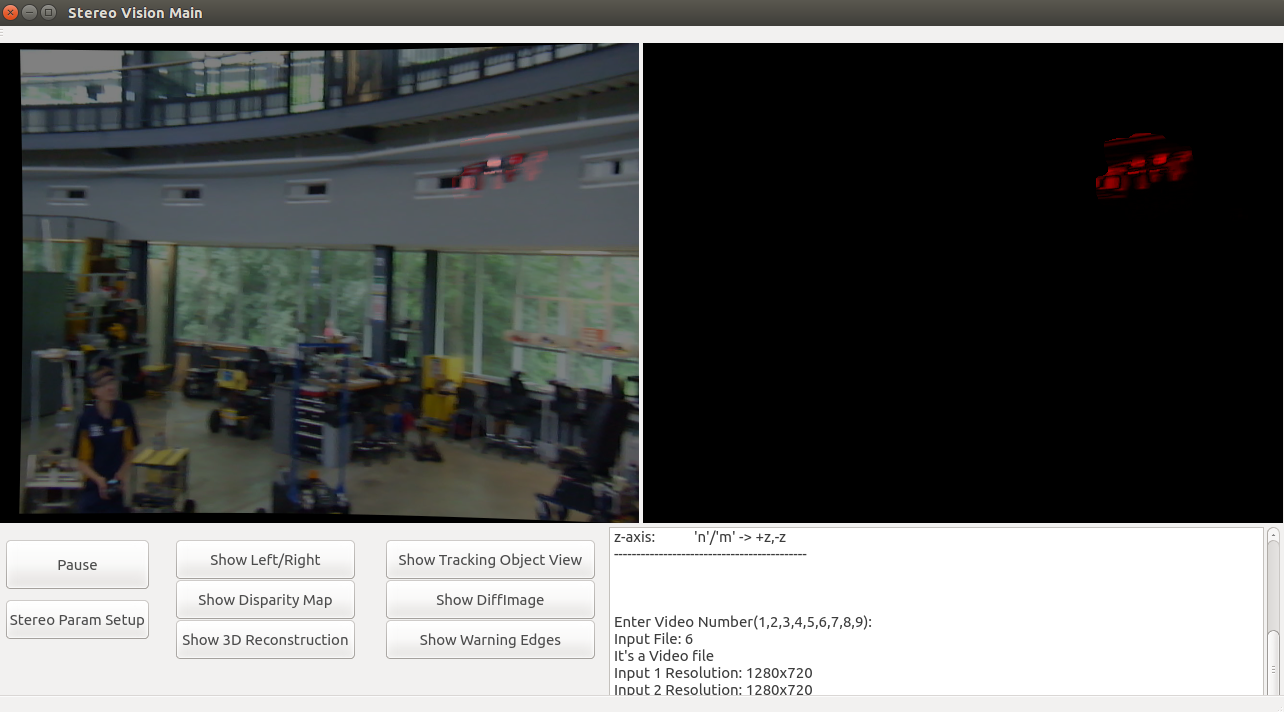
\includegraphics[scale=0.35]{./Resources/gui_showwarningedges_view.png}
 	\caption{Interface Gráfica - Visualização da Imagem resultante da adição da imagem à direita com a Imagem da Câmera Esquerda e Imagem resultante do processo de realce das bordas dos 
 	objetos em movimento próximos ao veículo}
 	\label{gui_showwarningedges_view}
\end{figure}


%-----------------------------------------------------------------------------------------------------------------------------------------------------------------------------------------------
\section{Comparação de Desempenho: Desktop x BBB x Jetson TK1}

Nesta seção, estão apresentados os resultados práticos das diferentes implementações dos métodos de visão estéreo nas plataformas abordadas. O Método utilizado foi o BM para a comparação das plataformas, visto que é o que requisita menor processamento dentre os outros métodos mais conhecidos (SGBM, BP, CSBP, AD Census, ...). A tabela \ref{resultsCPUGPU} abaixo, apresenta o resultado de desempenhos obtidos nas plataformas, apresentando comparativamente seu desempenho quando o processado utilizando CPU ou GPU/NEON (Caso da BBB).

\begin{table}[]
\centering
\caption{Desempenho atingido de cada plataforma utilizando o método de correspondências BM}
\label{resultsCPUGPU}
\begin{tabular}{c|c|c|ll}
\cline{2-3}
                                          & \textbf{CPU(FPS)} & \textbf{GPU/NEON(FPS)} &  &  \\ \cline{1-3}
\multicolumn{1}{|c|}{\textbf{Desktop}}    & 1                 & 1                      &  &  \\ \cline{1-3}
\multicolumn{1}{|c|}{\textbf{BBB}}        & 1                 & 1                      &  &  \\ \cline{1-3}
\multicolumn{1}{|c|}{\textbf{Jetson TK1}} & 1                 & 1                      &  &  \\ \cline{1-3}
\end{tabular}
\end{table}


%-----------------------------------------------------------------------------------------------------------------------------------------------------------------------------------------------
\subsection{Desktop}
\subsubsection{CPU}
\subsubsection{GPU}


%-----------------------------------------------------------------------------------------------------------------------------------------------------------------------------------------------
\subsection{BeagleBone Black(BBB)}
\subsubsection{CPU2}
\subsubsection{NEON}


%-----------------------------------------------------------------------------------------------------------------------------------------------------------------------------------------------
\subsection{Jetson TK1}
\subsubsection{CPU}
\subsubsection{GPU}